
Two tools for cryptographic protocol verification are going to be discussed: \href{https://prosecco.gforge.inria.fr/personal/bblanche/proverif/}{Proverif} and \href{https://tamarin-prover.github.io/}{Tamarin-Prover}. Tamarin-Prover will also be referred to as Tamarin for brevity.

\begin{figure}[!h]
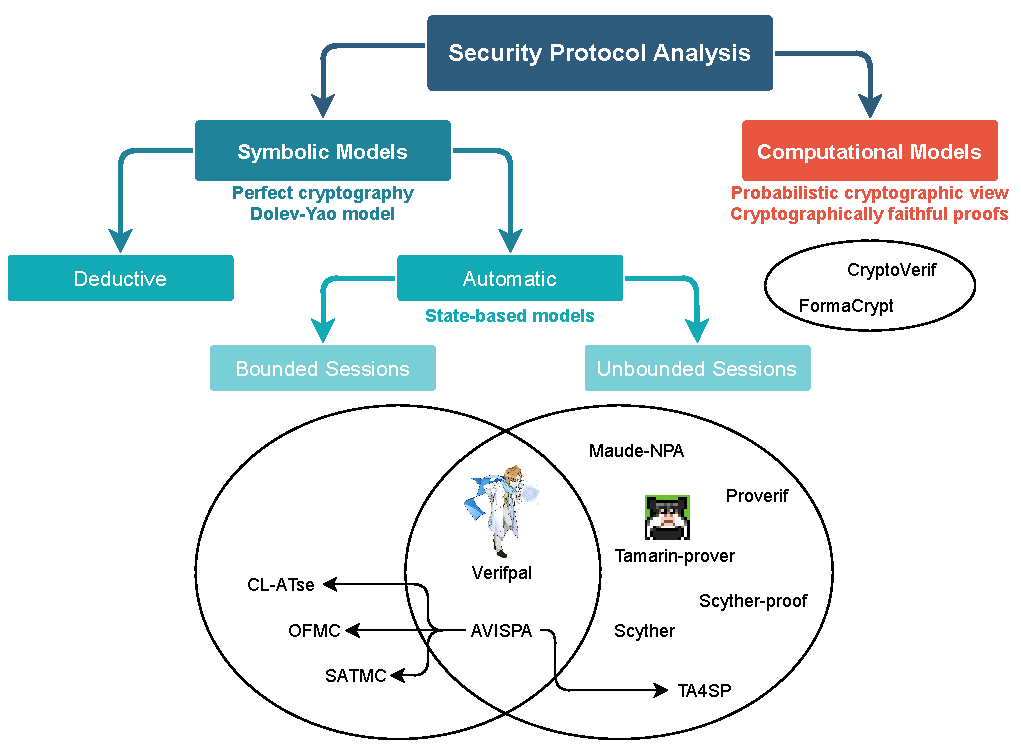
\includegraphics[scale=0.9]{symbolic-computational-model}
\centering
\end{figure}

\section{Proverif}
% TODO

\section{Tamarin}
In this section we will see an overview of Tamarin foundations and internal reasoning.
For a more in-depth description and further information, see the Tamarin foundations paper \cite{TamarinFoundations} or the extended foundations paper \cite{TamarinFoundationsExtended}.

\subsection{High level view}
First of all, let's have a look at an high level picture of Tamarin.

The security property model of Tamarin is based on multiset rewriting rules to specify protocols and adversary capabilities, a guarded fragment \cite{FragmentFirstOrderLogicPaper} of first order logic to specify security properties \footnote{Security properties will also be referred to as \textit{lemmas}.} and functions and equational theories to model the algebraic properties of cryptographic protocols \cite{TamarinFoundations}.

Given the rewriting rules, security properties and equational theories, Tamarin uses a novel constraint-solving algorithm which tries to validate or falsify lemmas.

Tamarin also offers builtin equational theories \cite{TamarinProverManual}. A brief overview will be given in subsection \ref{Proverif-and-Tamarin_Tamarin_Builtin-equational-theories}.

\subsection{Builtin equational theories}
\label{Proverif-and-Tamarin_Tamarin_Builtin-equational-theories}
A brief list of Tamarin built-ins is given below: \footnote{Only the builtin theories used in the analysis or the relevant ones will be described here. The full list is available in the Tamarin manual.}

\begin{description}[style=nextline]
    \item[hashing] defines a perfect hash function \textbf{h/1} \footnote{The writing \textbf{f/x} indicates that the function \textbf{f} has arity \textbf{x}.}
    \item[asymmetric-encryption] models a public key encryption scheme. It defines the following symbols:
    
    \begin{itemize}
        \item{\textbf{aenc/2}, used to model the encryption of a message with a public key}
        \item{\textbf{adec/2}, used to model the decryption of an encrypted message with a private key}
        \item{\textbf{pk/1}, used to derive a public key from a private key}
    \end{itemize}

    Functions are related by the equation \textbf{adec(aenc(msg, pk(sk)), sk) = msg}.

    \item[diffie-hellman] models Diffie-Hellman groups. It defines the following symbols:
    
    \begin{itemize}
        \item{\textbf{inv/1}, models the inverse of an element}
        \item{\textbf{1/0}, models the neutral element}
        \item{\textbf{\textasciicircum} and \textbf{*} symbols, models exponentiation and multiplication respectively}
    \end{itemize}

    The equational theory for this builtin is actually quite complex. For the sake of completeness, these are the related equations:
    \begin{itemize}
        \item{(x \textasciicircum y) \textasciicircum z = x \textasciicircum (y * z)}
        \item{x \textasciicircum 1 = x}
        \item{x * y = y * x}
        \item{(x * y) * z = x * (y * z)}
        \item{x * 1 = x}
        \item{x * inv(x) = 1}
    \end{itemize}
    % TODO: parla ancora un po' di quanto sia figo Tamarin che ha DH builtin!
\end{description}

\section{Comparison of Proverif and Tamarin}